\documentclass{sigchi}

% Use this command to override the default ACM copyright statement (e.g. for preprints). 
% Consult the conference website for the camera-ready copyright statement.


%% EXAMPLE BEGIN -- HOW TO OVERRIDE THE DEFAULT COPYRIGHT STRIP -- (July 22, 2013 - Paul Baumann)
% \toappear{Permission to make digital or hard copies of all or part of this work for personal or classroom use is 	granted without fee provided that copies are not made or distributed for profit or commercial advantage and that copies bear this notice and the full citation on the first page. Copyrights for components of this work owned by others than ACM must be honored. Abstracting with credit is permitted. To copy otherwise, or republish, to post on servers or to redistribute to lists, requires prior specific permission and/or a fee. Request permissions from permissions@acm.org. \\
% {\emph{CHI'14}}, April 26--May 1, 2014, Toronto, Canada. \\
% Copyright \copyright~2014 ACM ISBN/14/04...\$15.00. \\
% DOI string from ACM form confirmation}
%% EXAMPLE END -- HOW TO OVERRIDE THE DEFAULT COPYRIGHT STRIP -- (July 22, 2013 - Paul Baumann)


% Arabic page numbers for submission. 
% Remove this line to eliminate page numbers for the camera ready copy
% \pagenumbering{arabic}


% Load basic packages
\usepackage{balance}  % to better equalize the last page
\usepackage{graphics} % for EPS, load graphicx instead
\usepackage{times}    % comment if you want LaTeX's default font
\usepackage{url}      % llt: nicely formatted URLs
\usepackage{listings}
\lstset{breaklines}
\usepackage{tabularx}
\usepackage{algpseudocode}
% llt: Define a global style for URLs, rather that the default one
\makeatletter
\def\url@leostyle{%
  \@ifundefined{selectfont}{\def\UrlFont{\sf}}{\def\UrlFont{\small\bf\ttfamily}}}
\makeatother
\urlstyle{leo}


% To make various LaTeX processors do the right thing with page size.
\def\pprw{8.5in}
\def\pprh{11in}
\special{papersize=\pprw,\pprh}
\setlength{\paperwidth}{\pprw}
\setlength{\paperheight}{\pprh}
\setlength{\pdfpagewidth}{\pprw}
\setlength{\pdfpageheight}{\pprh}

% Make sure hyperref comes last of your loaded packages, 
% to give it a fighting chance of not being over-written, 
% since its job is to redefine many LaTeX commands.
\usepackage[pdftex]{hyperref}
\hypersetup{
pdftitle={SIGCHI Conference Proceedings Format},
pdfauthor={LaTeX},
pdfkeywords={SIGCHI, proceedings, archival format},
bookmarksnumbered,
pdfstartview={FitH},
colorlinks,
citecolor=black,
filecolor=black,
linkcolor=black,
urlcolor=black,
breaklinks=true,
}

% create a shortcut to typeset table headings
\newcommand\tabhead[1]{\small\textbf{#1}}


% End of preamble. Here it comes the document.
\begin{document}

\title{Crowdsourcing on In-building Routing System with Personal Preferences across Building Groups}

\numberofauthors{3}
\author{
  \alignauthor Junnan CHEN\\
    \affaddr{Waterloo, Canada}\\
    \email{j486chen@uwaterloo.ca}\\
  \alignauthor Henagzhi ZHANG\\
    \affaddr{Waterloo, Canada}\\
    \email{h246zhang@uwaterloo.ca}\\
}

\maketitle

\begin{abstract}
People travel inside building groups from a room in building A to another in building B frequently. Traditional routing systems usually provide the shortest routes between two coordinates consist of longitudes and latitudes, but do not have knowledge about building structures and detailed floor maps. These systems do not take users' personal preferences into account when suggesting routes as well. Such routes cannot meet people’s demand. In this paper, we introduce a new system, which provides in-building routes based on personal preferences across building groups.
\end{abstract}

\keywords{
	Crowdsourcing; In-building Routing; Personal Preferences; Mobile Interfaces; Concept of Association; Decision Tree.
}

\section{Introduction}

introduction
In our world, most people are living, working or studying in a group of buildings which could be company buildings, neighbourhoods or campus buildings. People go from one location inside the building-group to another every hour every day. Traditional route planning system provides routes between two coordinates consist of longitudes and latitudes, focusing on finding the shortest route, but does not have knowledge about the inside structures of buildings and floor-detailed environments, and does not take users' personal perferences into account when suggesting the routes. Those routes cannot provide enough details and personal options demanded by people.
For example, an employee may need to go to the coffee shop on the first floor of building B from his office on the third floor of building A several times a day. His route choices would be based on the weather condition and his physical condition. He would choose to go through the hallway between the two buildings if it rained or take the elevator if he feels tired. Traditional route planning system would only provide the shortest route from the exit of building B to the entrance of building A regardless of the building structures or floor environments, which cannot meet this employee's actual needs.


Here we want to introduce a new in-building routing system with persoanl preferences, a system with comprehensive knowledge of building structures, floor-level detailed maps, and relevant environments, which provides room-level detailed routes with personal preferences specified by the user. The focus of this system would be mapping the physical features of routes to human preferences which consist of physical requirement, personal feelings, emotional options and etc. The system shall collect route and preference data from people, and then analyze the relationships between human preferences and physical features.


Our system collect the trainning data, which are actual routes each has its personal preferences labeled, by crowdsourcing methods. Crowdsourcing has been successfully used in many fields. We provide an application on mobile devices, which encourages people to record their daily routes from one room location to another across building groups. Before they start to record routes, the application will ask the user about their personal feelings today (e.g. Are you hurry now? or Are you feeling tired now?), their special demands for the following route (e.g. Will you pass Tim Hortons on your way? or Do you need to use the bathroom on your way?) as well as some weather conditions (e.g. Is it sunny out side? or Is it snowing now?). Once the users finish the questionares, they will be presented an interface for them to record their routes. During the recording process, the application collects physical data of the route in the form of points on the floor map inputted by the user. 


Our system will analyse the routes collected and the corresponding physical features of a particular route (e.g. the number of stairs, number of turns) with personal preferences such as physical requirement, personal feelings, and emotional options provided by the user. We will construct our model using the concept of decision tree. The model is trained by the collected data and will be able to predict the best route given a set of personal preferences.


Our final product aims to generate the proper routes upon request. Using this product, the user could specify two room locations, together with one or more personal preferences. Then, the system will run the model and return the most satisfying route. The system will display the route on the screen for the user. 


In this paper, we describe the design of the courdsourcing routes collecting method, the feature analysing method and route generating system. We test the system with University of Waterloo campus building groups. We provide the test results, the detailed evaluation of our system and the future work.


\section{RELATED WORK}

During the system design process, we reviewed literature related to our ideas. The Kimono ~\cite{huang2005kimono} is a knowledge sharing system, which presents the concept of association. Our in-building routing system uses this idea as well; for example, each route collected in the crowdsourcing stage is associated with a set of personal preferences specified by the user. One of the prior works we reviewed has the similar idea since it ~\cite{heimerl2012communitysourcing} includes a physical kiosk as well. In addition, the physical kiosks ~\cite{heimerl2012communitysourcing} are used for crowdsourcing. Since our system collects in-building routes with personal preferences from our users, crowdsourcing plays a significant role here, and crowdsourcing needs to be studied from the prior work ~\cite{howe2006rise,ipeirotis2014quizz,alt2010location}. Since our system requires users to record routes on the map displayed on the screen and provide inputs through the questionnaire, user interface designs need to be taken into our consideration. Some prior works ~\cite{della2013crowdsourcing,vaataja2011crowdsourced} provide us with very helpful results for our system design. Our results are based on decision trees. In order to have some insights about decision trees, we reviewed and studied related work ~\cite{su2006fast,quinlan1987simplifying}. In this section, we discuss how prior work helps us develop our in-building routing system with personal preferences across building groups. 


\subsection{Concept of Association}

The Kimono paper ~\cite{huang2005kimono} presents a system, which extends the function of an information kiosk. The method they used in order to achieve the extension is to allow interactions between a kiosk and a mobile device, such as a smartphone. We know that a kiosk is usually a physically located machine displaying information. A user could stand in front of a kiosk, and touch the screen to select information of his or her interest. The information from the kiosk is relevant to the particular event at its location. Some disadvantages of a kiosk can be seen. For example, the kiosk lacks mobility, and it’s difficult to add more information to it.


To conquer these inflexibilities, the main idea introduced in the paper ~\cite{huang2005kimono} is to allow interactions between a mobile device (such as a smartphone) and a kiosk. People are familiar with smartphones as they use phones every day. Functionalities of a smartphone include taking pictures, taking notes, recording voices, and so on. Through these various ways, a person can easily create new contents at any time at his or her current location. Then he or she can associate the newly created contents with other selected contents or events presented on the kiosk. By uploading the new contents and its associations, other people can therefore have access to them.


The Kimono system ~\cite{huang2005kimono} described in the paper is designed specifically for researchers attending a conference. A number of kiosks are placed in the lobby of the conference. They all display the same information relevant to the event, such as conference locations, routes to the airport, hotels, etc. Changes of talk schedules and meal plans are posted on the kiosks as well. Participants of the conference use the touch panel display of a kiosk to select information interested in. Then the information selected is transferred to his or her smartphone. On the smartphone, the program will alert the user about the next event and other relevant details such as starting/ending time, room location, routes to the destination, etc.


While attending a lecture at the conference, one can use their smartphones to record notes in the form of text, image, video, or audio. Then they associate newly created notes with selected event or items such as papers or posters presented at the conference. People can also exchange notes with each other directly between two mobile devices, or post the notes they took on the kiosk. For those users who previously downloaded information from the kiosk to their smartphones, if the information downloaded has changed, the updates will be copied to the mobile devices through the system when the next synchronization occurs. 


The main insight we learned from the Kimono ~\cite{huang2005kimono} is the concept of associations, which makes the organization of data and synchronization much more simple. Users can get information of his or her interest displayed on the screen and associated information on the smartphone. New information can be created by the user, associated with other relevant information, and made available to others.


For our in-building routing system with personal preferences across building groups, the concept of association is utilized. During the crowdsourcing stage, users record their routes while walking to the destination, and later associate personal preferences or features with the route they just recorded. Personal preferences in our system include physical requirements, personal feelings, emotional options, etc. By associating personal preferences with the routes, the system could provide in-building routes with particular personal preferences specified by a user, and later collect ratings from the user about the routes suggested. 

\subsection{Crowdsourcing}

We can see that a lot of researches and experiments are conducted in prior works ~\cite{heimerl2012communitysourcing,alt2010location} in the area of crowdsourcing. Here we discuss the paper ~\cite{heimerl2012communitysourcing}, in which crowdsourcing concepts are presented and extended as communitysourcing. What we know is that crowdsourcing involves division and assignment of tasks to a number of online users. In order to have better quality work, the kiosk is used to attract the right crowds to perform tasks. In this case, the right crowds are required to be knowledgeable enough in the corresponding task domain assigned to them. The result the paper showed is that the crowdsourcing system was able to perform the grading task more accurately than traditional grading.


What we did is to incorporate the idea of crowdsourcing into our system. That is, we let crowds generate routes with personal preferences through our system. As the system provides in-building routes across building groups on campus, the potential crowds we are interested in are students, teachers, and staffs. One reason is that they are familiar with the building structures and floor-detailed environments, and therefore the quality of crowdsourced routes is greatly improved. Another reason is that we could obtain enough route data in a relatively short period of time through the crowdsourcing stage. Furthermore, during the crowdsourcing stage, the system could capture a particular set of preferences associated with a route, and later suggest this route upon requests of same or similar preferences in the set.


\subsection{User Interface}

Since we require the routes to be recorded when users walk to their destinations, our system provides an interface on both computers and mobile devices. The user gets access to our system on the screen in the beginning of his or her journey. Partial map centered at his or her current position is displayed. The user periodically marks his or her next new position along the way to the destination, and the map accordingly centers at the newly marked position. A questionnaire is displayed to request his or her personal preferences associated with the recorded route before the user starts recording.


The questions on the questionnaire are asked before the recording process. The questionnaire of our system helps to collect the personal preference data with the crowdsourced routes of our interest. After thinking of what kinds of questions should be asked, we have the questions such as the weather conditions, the fatigue level, pass coffee shop or not, hurry level, and etc.


When designing such a crowdsourcing interface, we need to think about whether our user interface or task design is effective on both computers and mobile devices. We reviewed the prior paper ~\cite{della2013crowdsourcing} to gain better understandings and insights about crowdsourcing user interfaces and task designs for mobile users.


The main question in the paper ~\cite{della2013crowdsourcing} the author trying to answer is “Which crowdsourcing platforms and which kinds of tasks are more adequate to mobile devices”. It turns out that some of those inadequacy issues are superficial, and they can be resolved by providing better user interfaces and/or better crowdsourcing task designs. Several typical reasons for such inadequacy issues on mobile phones are found as well, such as redundant task description, unsupported formats of audio, scrolling problem, layout problem in a small display, and so on.  


For our system, we also try to conquer these problems by designing simple tasks, requesting simplified inputs, providing concise interfaces, etc. Our system knows the building structures and all of the floor maps. Users records routes through their mobile devices while walking. Partial map centered at the current position is showed, and the user marks the next point along the journey. Upon request of a route with personal preferences specified by a user, the system provides in-building routes and collects ratings for the suggested route afterwards. Several benefits can be seen in our system. For example, instead of keeping track of the entire route walked, the user only needs to mark the next new point by touching the screen every time they move as the partial map will always centered at his or her current point. After gathering point information inputted by the user, the system itself can generate the corresponding route. By displaying only the partial map instead of the entire floor map, we successfully resolve the bad layout problem on small portable screens.


\subsection{Decision Tree}

Our results are based on decision trees. As described in the previous section, our system provides users with an interface through which users perform question answering and route recording tasks. The system requires users to answer a questionnaire before they start to record their in-building routes during the crowdsourcing stage. The questionnaire here in the system is used to collect personal preference data associated with the routes recorded. And decision trees are then built accordingly. 


We built several graphs of decision trees. What we did was the review of several prior works ~\cite{su2006fast,quinlan1987simplifying} involving the decision trees. A decision tree provides us with support in decision-making. It is known as a tool, which uses a tree like graph or model of decisions and their possible consequences. A decision tree is a useful technique, which learns a model from a provided data set inductively. In order to build a decision tree, we need to be clear about the structure of a decision tree. The tree structure consists of internal nodes, branches, and leaf nodes. We describe each of the above in turn. Each of the internal nodes is a test on an attribute from our crowdsourced data. Each of the branches represents the result from an internal node. Lastly, a leaf node can be seen as a class label. Three types of nodes are in a decision tree. They are decision nodes, chance nodes, and end nodes. The algorithm is shown to readers through a decision tree. 


Existing algorithms are introduced in early papers ~\cite{breiman1984classification,quinlan1986induction} to help build decision trees. These algorithms ~\cite{breiman1984classification,quinlan1986induction} build decision trees from the given set of training data. Top down structures are built, partitioning instances into different classes. The splits of instances are based on different attribute values. The algorithm from early work ~\cite{breiman1984classification} uses Gini index to select the splitting attribute. The Gini impurity measures how often a random element from a data set is incorrectly labeled if it was randomly labeled according to the distribution of labels in the subset. Specifically, the Gini impurity is the summation of fi times (1-fi) where fi is the fraction of elements labeled with i.


Decision trees are traditionally drawn manually. However, they can grow to very large trees, which makes it difficult for a person to draw by hand. Here, we used a specialized package in Python to generate decision tree graphs for us. Our goal is to have a model that learns from the data gathered and later makes predictions on some variable of interest. In the graphs we created, colored nodes according to their classes together with explicit variable names are shown. 


Decision trees are commonly utilized in many analytical procedures. What we learned from prior work are a number of advantages of such a decision support technique as follows. For example, a decision tree is relatively easy to understand and interpret, and it requires little data preparation. Furthermore, it allows adding new cases, and can be combined with other decision support techniques. The cost of prediction on a targeted variable using the tree is logarithmic in the training data size.

\section{SYSTEM DESCRIPTON}

Our system shall be built with knowledge of building structures and floor-level detailed maps of a building group. The main problems that this system is trying to address are collecting routing data with corresponding personal preferences, constructing the routing model based on the collected data. 


The route suggestion problem can be considered as a classification problem. The input data we get from the users are their current status (e.g. if they are tired) and environment conditions (e.g. is it sunny). Our goal is to generate an most suitable route based on all of these variables. For example, if the users are tired, a route using elevators should be more suitable than one which uses stairs intuitively. Since most of the status and conditions we currently consider, like if the user is tired or if the user needs to use a printer, are discrete variables. Taking this into considerations, we determine that a decision tree should be a good option.


\subsection{Basic workflow}

Our basic workflow of the modeling procedure is shown in Figure~\ref{fig:systemflow}

\begin{figure*}[!h]
\centering
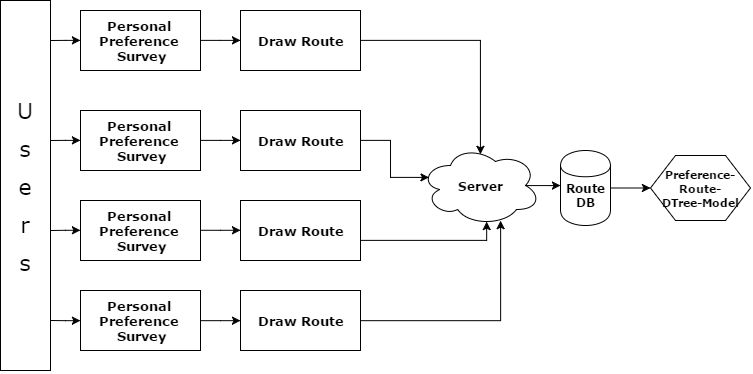
\includegraphics[width=2.0\columnwidth]{pics/work-flow.png}
\caption{System flow chart}
\label{fig:systemflow}
\end{figure*}

The modeling procedure mainly consists of two parts:
\begin{itemize}
\item Training data collecting - Crowdsourcing
\item Decision tree constructing
\end{itemize}

\subsection{Training data collecting - Crowdsourcing}

To build a model for the route suggestion problem, we first need to collect data for training decision trees by taking advantage of crowdsourcing.


Crowdsourcing basically has two aspects, to break a large-scaled complex problem into several pieces of sub-problems, and to involve human efforts to solve or help solve the sub-problems which could be time saving because the solving of sub-problems are highly paralleled. Therefore, we found crowdsourcing has the properties which fit the demand of our system perfectly. In the data collection process, we apply crowdsourcing concept by having our participants to record the routes and score the preference options for that route.


The training data collection contains two steps:
\begin{itemize}
\item Survey - Uses are asked finish a survey about their status and environment conditions.
\item Route drawing - Users are asked to draw a path based their answers to the former survey.
\end{itemize}

\subsubsection{Survey}

The questions and possible answers are in the survey are listed in table~\ref{table:survey_questions}. We convert these answers to a preference vector. From the table, we can see that the values of each element of the vector are discrete. The questions list are far from complete. One potential future work is that we can add more questions based on users’ feedback in crowdsourcing.
\begin{table}
  \centering
  \caption{Survey questions and answers}
  \label{table:survey_questions}
  \begin{tabularx}{0.5\textwidth}{|X|l|}
    \hline \hline
    Questions & Answers \\\hline
    Is it sunny outside? & Yes/NO \\\hline
    Is it cloudy outside? & Yes/NO \\\hline
    Is it rainy/snowy outside? & Yes/NO \\\hline
    Do you feel tired now? & Yes/NO \\\hline
    Do you want to go to Tim Hortons on your way? & Yes/NO \\\hline
    Do you want to go to bathroom on your way? & Yes/NO \\\hline
    Do you want to avoid crowds at a particular time (e.g. heavy crowds outside MC2065 when class ends, crowds when special events take place, etc.)? & Yes/NO \\\hline
    Are you curious of the floor environment (e.g. first time visit, etc.)? & Yes/NO \\\hline
    Do you need the printer on your way? & Yes/NO \\\hline
    Are you hurry or not through this walk? & Yes/NO \\\hline
    Do you want some fresh air on your way? & Yes/NO \\\hline
    \hline
  \end{tabularx}
\end{table}

\subsubsection{Route drawing}

The users are asked to draw the routes on the maps of each floor. On each map, we marked some special places, like the restrooms, Tim Hortons etc. These marks can help users to plan their route according to their answers (e.g. if they want to grab a cup of coffee). After the users finished their drawing, we will store this route in our server. The route data is in JSON format. One example is:


\begin{lstlisting}
"data":{
  "paths":[
            [
              {"mapURL":"maps/dc1.png","pointList":[{"x":774.6552269835852,"y":834.1966612816371}]},
              {"mapURL":"maps/dc2.png","pointList":[{"x":677.4289260557916,"y":568.6845449649974}]}
            ]
          ],
  "id":["1449207710639"]
}
\end{lstlisting}

After that, we will do analysis on the route data. We analyze each route to derive several physical properties:
\begin{itemize}
\item Number of stairs
\item Times of using elevators
\item Times of exiting buildings
\item If going near Tim Hortons
\item If going near a printer
\item If going a restroom
\item The distance
\item If the route never goes outside
\end{itemize}

A vector of the eight properties is called a physical property vector. A physical property vector should be related to the preference vector.


In summary, for each user, the data we collect is illustrated in Figure~\ref{fig:element-detail}.

\begin{figure}[!h]
\centering
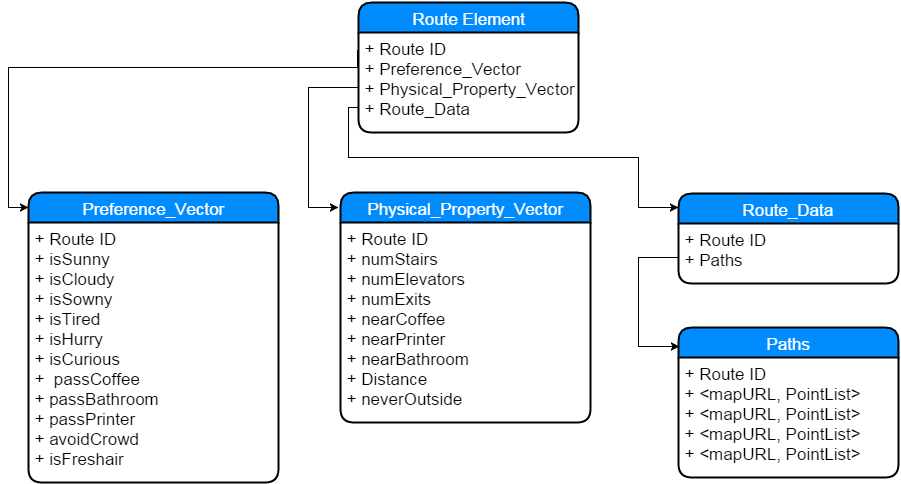
\includegraphics[width=1.0\columnwidth]{pics/element-detail.png}
\caption{System flow chart}
\label{fig:element-detail}
\end{figure}

\subsection{Decision tree constructing}

A decision tree is a flowchart-like structure in which each internal node represents a \"test\" on an attribute (e.g. whether a coin flip comes up heads or tails), each branch represents the outcome of the test and each leaf node represents a class label (decision taken after computing all attributes). The paths from root to leaf represents classification rules.


In decision analysis a decision tree and the closely related influence diagram are used as a visual and analytical decision support tool, where the expected values of competing alternatives are calculated.


We use Scikit-Learn, a python machine learning library, to construct these decision trees. The scikit-learn library is a powerful machine learning toolkit. Besides decision tree construction algorithms, it also provides a useful interface to generate a visual representation of the decision tree.


Using the training data we collected in the former step, we build two types of decision trees:
\begin{itemize}
\item physicalPropertyDecisionTree
\item routeSuggestionDecisionTree
\end{itemize}

\subsubsection{physicalPropertyDecisionTree}

This tree  is used to predict the desired physical properties by the users based on their current status and environment conditions. For each physical property, we build a decision tree independently. The reason we build a separate decision tree for each physical property is because we want to generate a physical property vector which doesn’t happen in the data collection step. If we build a decision tree for the entire physical property vector, all leaf nodes of the decision tree represents a vector we have met in the collection step.


\subsubsection{routeSuggestionDecisionTree}

This tree is used to predict the most suitable route according to the physical property vector. With this decision tree, given a physical properties requirement (e.g. the route should pass by a restroom), we are able to suggest a route which match the requirement as much as possible.

\subsection{Route Suggesting Procedure}
In the route suggesting procedure, the basic workflow is described in Figure~\ref{fig:route-suggest-work-flow}.

\begin{figure}[!h]
\centering
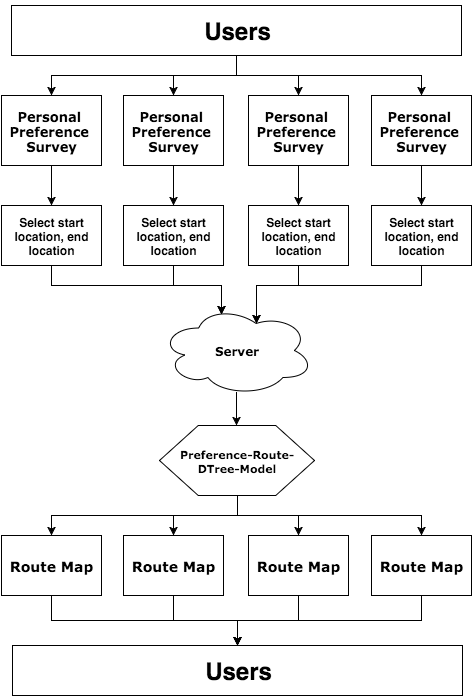
\includegraphics[width=1.0\columnwidth]{pics/route-suggest-work-flow.png}
\caption{System flow chart}
\label{fig:route-suggest-work-flow}
\end{figure}

The suggested route is generated based on the user’s answers to the scenario form. The generation process consists of two steps.

\subsubsection{Step 1: Physical Property Vector Generation}
The data we received from the user, which is in the same format of the survey data in modeling procedure,  is a preference vector. From the vector, we can derive the physical properties the user desires. For each property, we use the corresponding physicalPropertyDecisionTree to predict an estimated value. These values form a physical property vector.

\subsubsection{Step 2: Suggested Route Generation}
We have already generated a physical property vector in step 1. With this vector, the routeSuggestionDecisionTree can be used to generate a route suggestion.

The pseudocode for the route suggesting algorithm is:
\begin{algorithmic}\footnotesize
  \Function{routeSuggestion}{scenarioData}
    \State preferenceVector$\gets$\Call{parse}{scenarioData}
    \For{0 $\leq$ i $<$ numOfPhysicalProperties}
      \State physicalVector[i]$\gets$physicalDT[i].predict(preferenceVector) \EndFor
    \State \Return routeDT.predict(physicalVector)
  \EndFunction
\end{algorithmic}

\section{EXPERIMENT}

In this section, we explain how we execute the crowdsourcing to collect data for training the model based on decision tree algorithms.


\section{Conclusion}

It is important that you write for the SIGCHI audience.  Please read
previous years' Proceedings to understand the writing style and
conventions that successful authors have used.  It is particularly
important that you state clearly what you have done, not merely what
you plan to do, and explain how your work is different from previously
published work, i.e., what is the unique contribution that your work
makes to the field?  Please consider what the reader will learn from
your submission, and how they will find your work useful.  If you
write with these questions in mind, your work is more likely to be
successful, both in being accepted into the Conference, and in
influencing the work of our field.

\section{Acknowledgments}

We thank CHI, PDC and CSCW volunteers, and all publications support
and staff, who wrote and provided helpful comments on previous
versions of this document.  Some of the references cited in this paper
are included for illustrative purposes only.  \textbf{Don't forget
to acknowledge funding sources as well}, so you don't wind up
having to correct it later.

\balance

\bibliographystyle{acm-sigchi}
\bibliography{report}
\end{document}
